\chapter{Prosessdokumentasjon}
\lettrine[lines=2]{I}{} følgende kappitel beskriver vi hvordan hele utviklinsprosessen for protitypene har foregått. Hensikten er at man skal illustrere hele prosessen fra idé, mockup til hi-hi prototype klar for brukertesting. Kapitlet består av mange for å på enklest muli måte ilustrere prosessen. for eventuell beskrivelse av funksjonalitet av de inngående moduler som er synlige på bildene henvises til appediks \ref{app:funksjonalitet}.

\marginpar{
Test for sitering av kilder.\cite{forelesning:tulpesh}\cite{book:utforming}\cite{book:desintsystems}
}


\section{Første utkast}
Etter at idéen om hva vi skal jobbe med var klar og diskutert tok det ikke lang tid før vi ble enige om hvordan vi skal sette sammen vårt forslag til en helhet. Hele gruppen var tydelig på at vi ønsker i stor gra å benytte oss av en løsning som baserer seg tydelig på noen av gestalt prisnipper.
Det som var spesielt viktig var at man deler opp de forskjellige moduler i flere undermoduler slik at de bilder en visuell og logisk helhet. 

\reversemarginpar{Støtteord:
Usability (brukbarhet): konsistens, brukerkontroll, passende presentasjon.
}

\marginpar{Viktige prinsipper:
feedback, constraints (bruker får ikke gjøre feil), affordances
}

\begin{figure}[ht]
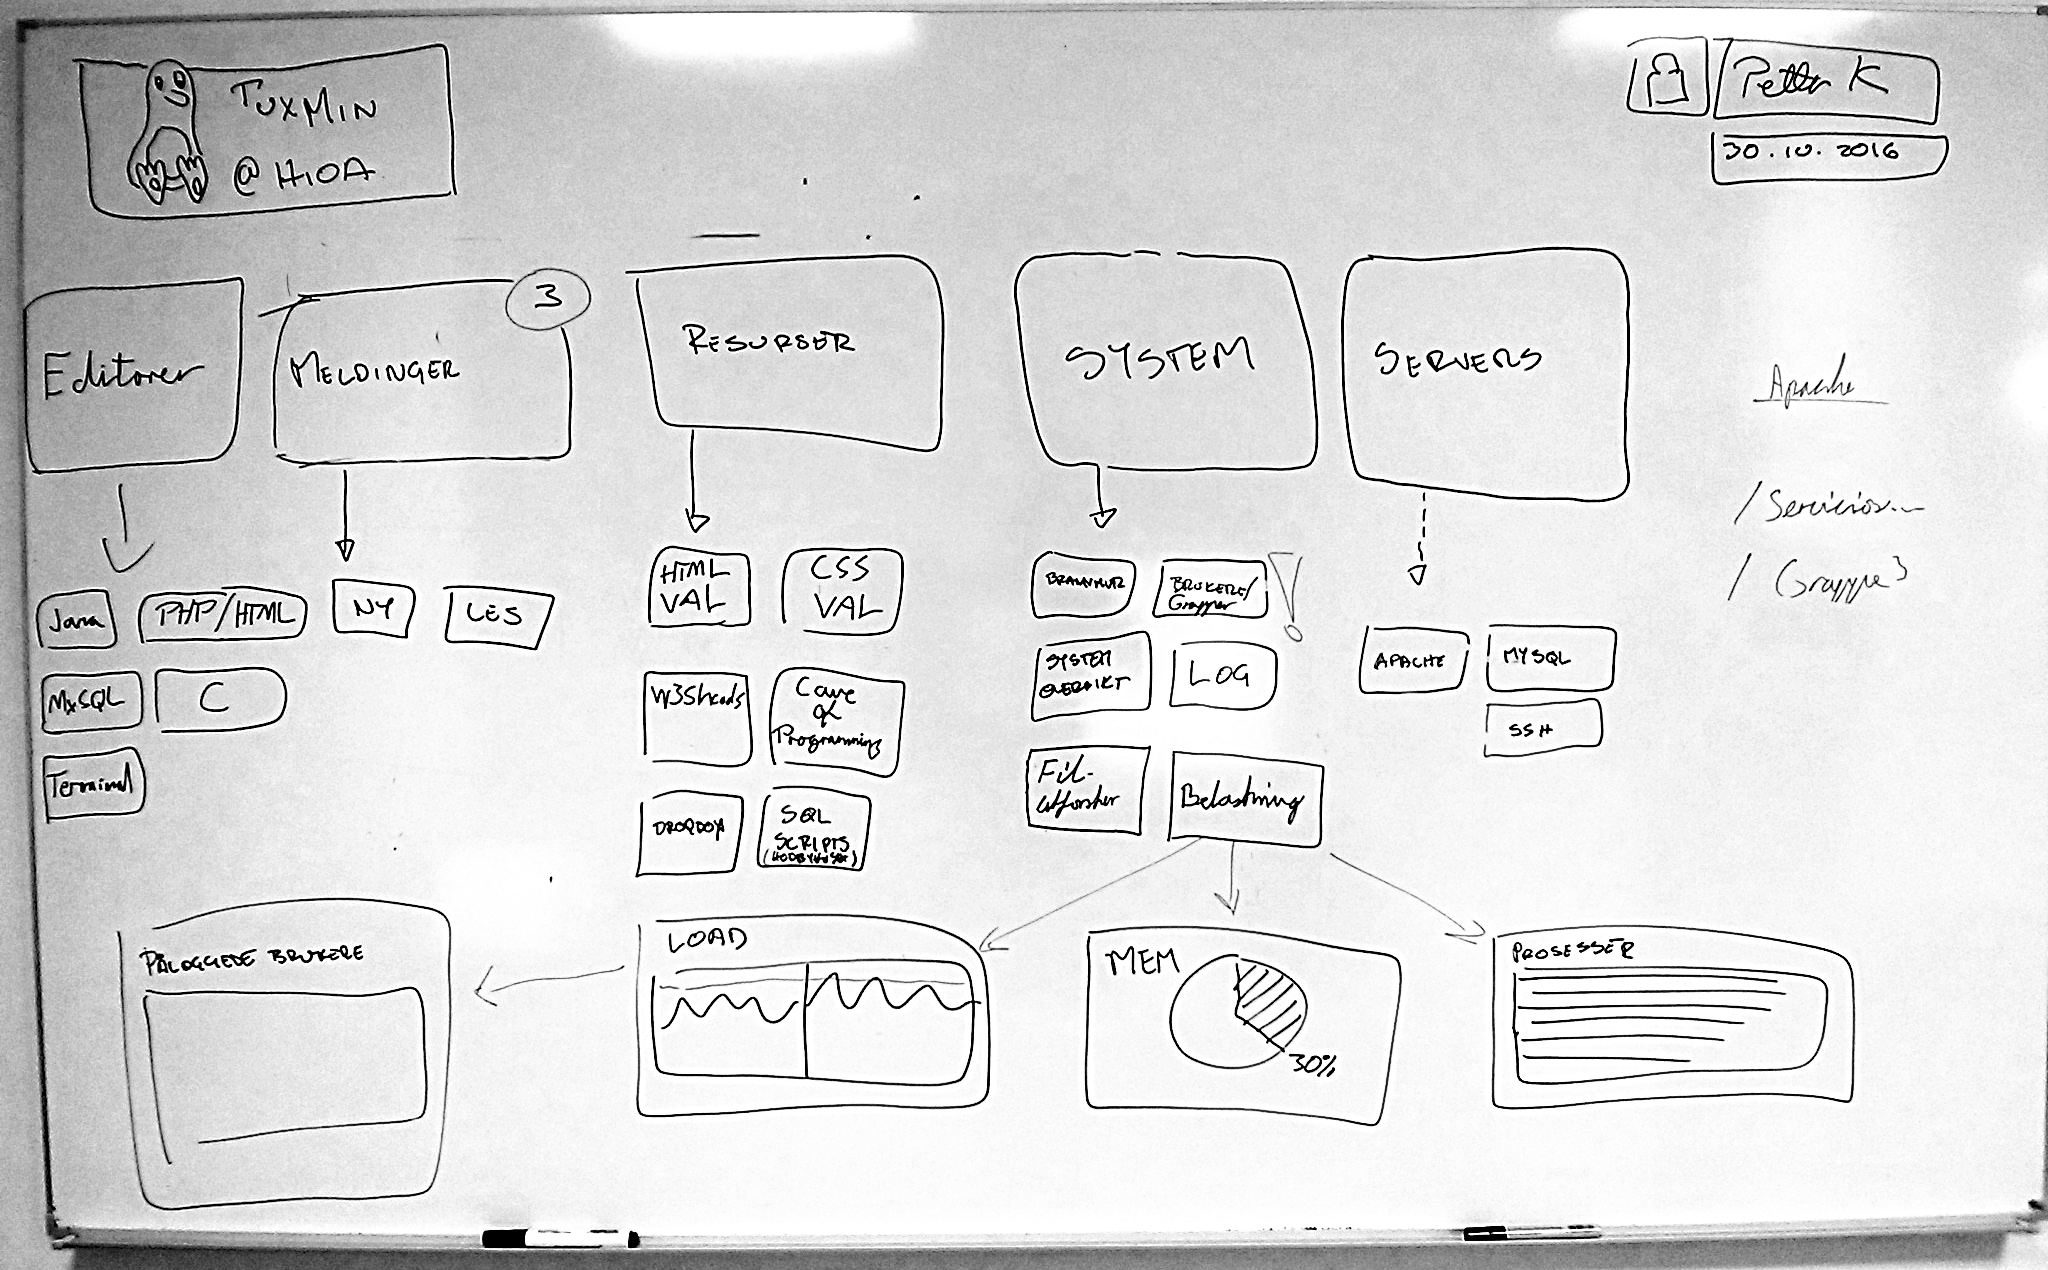
\includegraphics[width=\textwidth,height=\textheight,keepaspectratio]{./img/prosessdokumentasjon/foersteutkast/foerste.jpg}
\caption[Første utkast]{Første utkast over brukergrensesnittet.}
\label{fig:foersteutkast}
\end{figure}

\section{Low-fi prototype}

\section{Hi-fi prototype}

\section{Kriterier og avgjøresler}
Fokuser på alle valg som ble tatt. Hvilke kriterier og 
prinsipper i faget ligger bak avgjørelsene? 

Her kan vi skrive om hvorfor vi har akkuratt valgt Linux. Hvorfor skal løsningen være webbasert og hvorfor skal den kjøres i en virtuell maskin? Og så andre kriterier og avgjøresel som vi har tatt under veien. 